\documentclass[12pt]{article}

\usepackage{amsmath}
\usepackage{amsfonts}

\usepackage{graphicx}
\usepackage{subcaption}

\begin{document}

The problem setting:\\
 We have a simulation of the dynamical system that is governed basically by a single parameter,­ the rate of switching.
 %
 Depending of the value of this parameter, this system dynamics range between heat equation dynamics and wave equation dynamics. 
 %
 In the heat equation dynamics, the initial conditions play very little role and the system dynamics over time are dominant. 
 %
 In the wave equation dynamics, the initial conditions play a significant role and the dynamics over time are less important.


Contribution: 
\begin{enumerate}
\item We demonstrate that an essential component of our analysis is working with the right observers (histograms/ensumble rather than a single position of a particle) and with the right metric between those observers (EMD).
%
\item We demonstrate that we recover the right factors that control the dynamical system, depending on the mode (In heat eq. mode ­ first recover the temporal dynamics, second the initial conditions; In wave eq. mode ­ first recover the initial conditions, second the temporal dynamics). In particular, these two components have a completely different ``nature” ­ for example, in this case, one parameter (initial condition) is governing the entire trajectory and the other parameter (dynamics) is governing the ``step­--by­--step" time evolution (within each trajectory).
\end{enumerate}

\section{Introduction}

\section{Problem formualtion}

\subsection{Chemotaxis ``story''} 
We look at a model of a stochastic velocity jump process that arises in models of chemotaxis \cite{...}.

\subsection{Stochastic particles}

We have a collection of $N$ particles, each of which has a position and velocity. 
%
Let $x_i(t)$ and $v_i(t)$ denote the position and velocity, respectively, of particle $i$ at time $t$.
%
The velocity of each particle is either $\pm s$, where $s$ is the speed. 
%
We initialize the particles such that
\begin{eqnarray}
x_i(0) & = 0 \\
\mathbb{P} \{ v_i(0) = +s \} & = p
\end{eqnarray}
where $p$ is some probability.
%
The velocity of each particle randomly switches between $\pm s$ following an (independent) Poisson process with rate $\lambda$.

We simulate this stochastic velocity jump process for $N=1000$ particles, and $p \in [0.1, 0.9]$.
%
We simulate the process for $t \in [0, 10]$, and record the positions of each particle at regular time intervals.
%
Let $X_{p, \lambda, s}(t)$ denote the vector of positions of the particles at time $t$ with initial right probability $p$, switching rate $\lambda$, and speed $s$.
%
We will consider two sets of simulations.
%
In one set, $\lambda = 1$ and $s=1$, and in the other set, $\lambda = 400$, and $s=20$.


\subsection{Partial differential equations}

Let $\rho(x, t)$ denote the probability density of the particles, and let $\rho^-(x, t)$ and $\rho^+(x, t)$ denote the probability density of the left and right moving particles, respectively.
%
It can be shown that, as $n \rightarrow \infty$, $\rho(x, t)$ obeys the following set of partial differential equations (PDEs)
\begin{eqnarray} \label{eqn:coupled_pdes}
\frac{\partial \rho^+}{\partial t} + s \frac{\partial \rho^+}{\partial x} & = -\lambda \rho^+ +\lambda \rho^- \\
\frac{\partial \rho^-}{\partial t} - s \frac{\partial \rho^-}{\partial x} & = \lambda \rho^+ -\lambda \rho^- 
\end{eqnarray}
%
Alternatively, \eqref{eqn:coupled_pdes} can be written as one, second--order PDE
\begin{equation} \label{eq:second_order_pde}
\frac{\partial^2 \rho}{\partial t^2} + 2 \lambda \frac{\partial \rho}{\partial t} = s^2 \frac{\partial ^2 \rho}{\partial x^2}
\end{equation}
%
We assume that $s^2/\lambda = D$ is constant.

\subsection{Asymptotic mode analysis}  \label{subsec:mode_analysis}

We will consider two regimes of simulation.
%
When $\lambda \rightarrow 0$ is small, one can see that the right-hand side of \eqref{eqn:coupled_pdes} tends to 0. 
%
Therefore, \eqref{eqn:coupled_pdes} becomes two uncoupled wave equations.
%
When $\lambda \rightarrow \infty$, $\frac{\partial^2 p}{\partial t^2} \rightarrow 0$ and \eqref{eq:second_order_pde} approaches the heat equation. 
 
\section{Methods and Analysis}

\subsection{Diffusion maps}

\subsection{Earth mover's distance}

\section{Results}


\begin{figure}[htb]
\begin{subfigure}{0.5\textwidth}
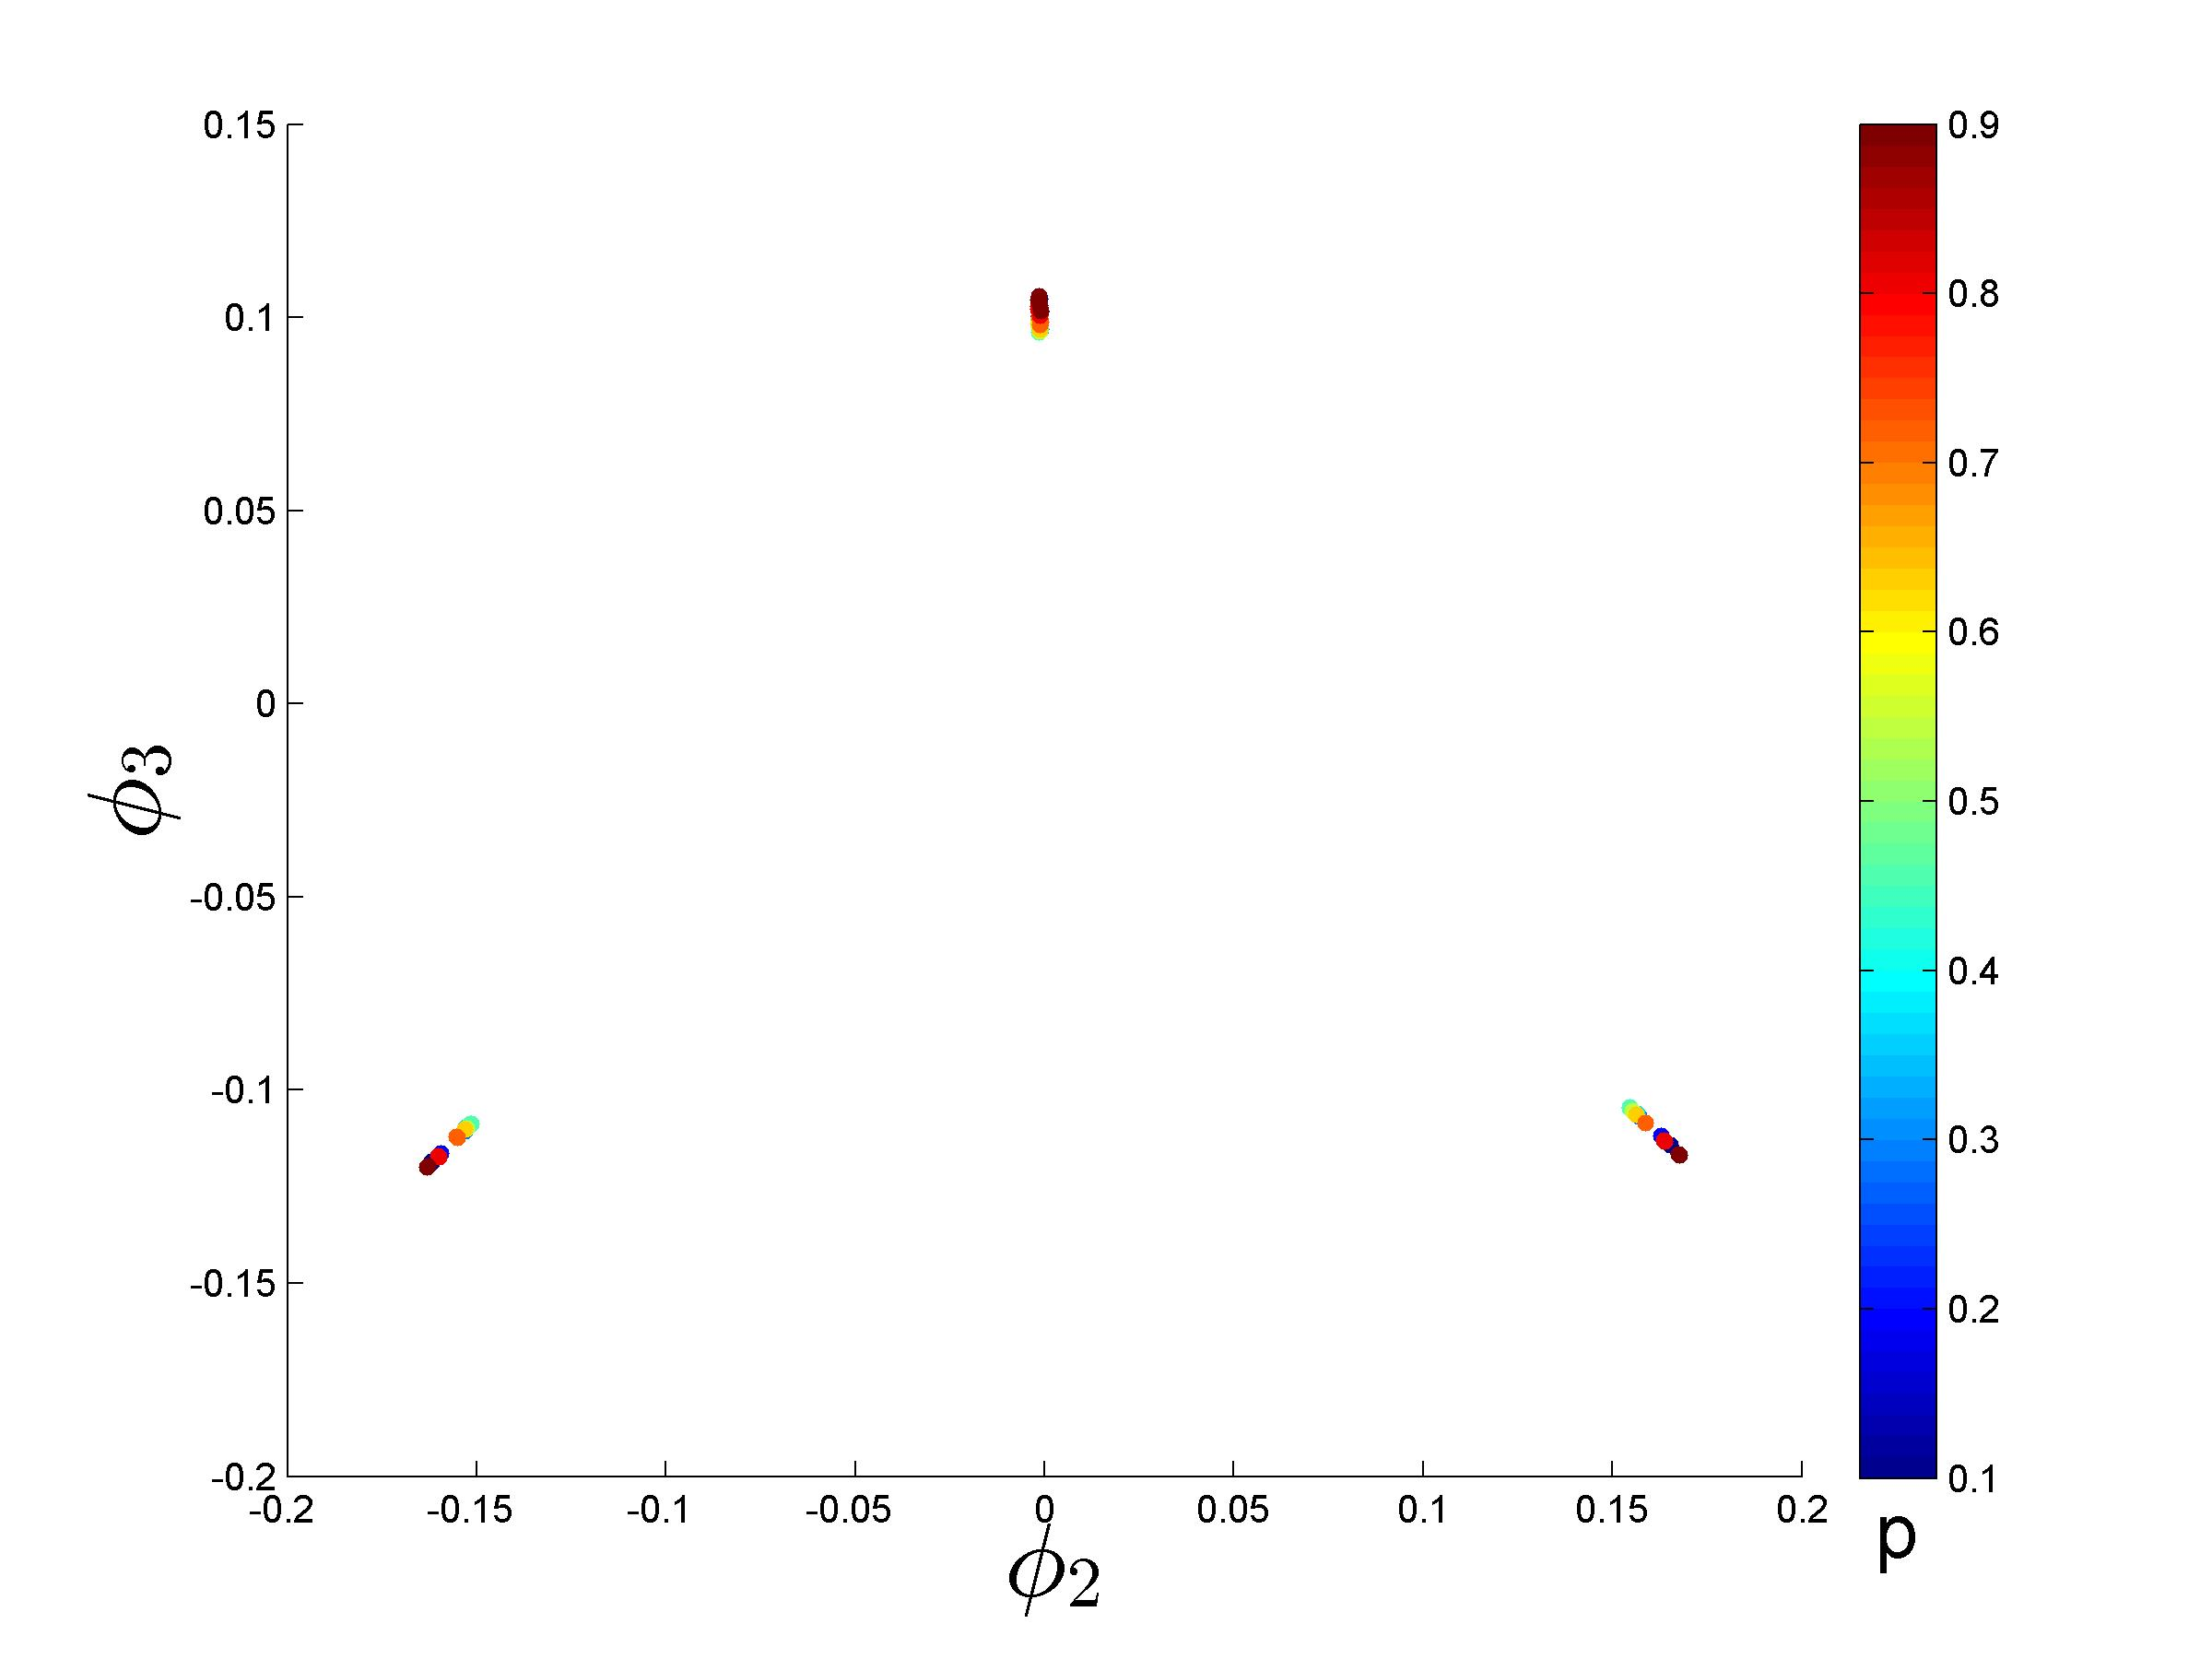
\includegraphics[width=\textwidth]{rawhist_p_1}
\caption{}
\end{subfigure}
\begin{subfigure}{0.5\textwidth}
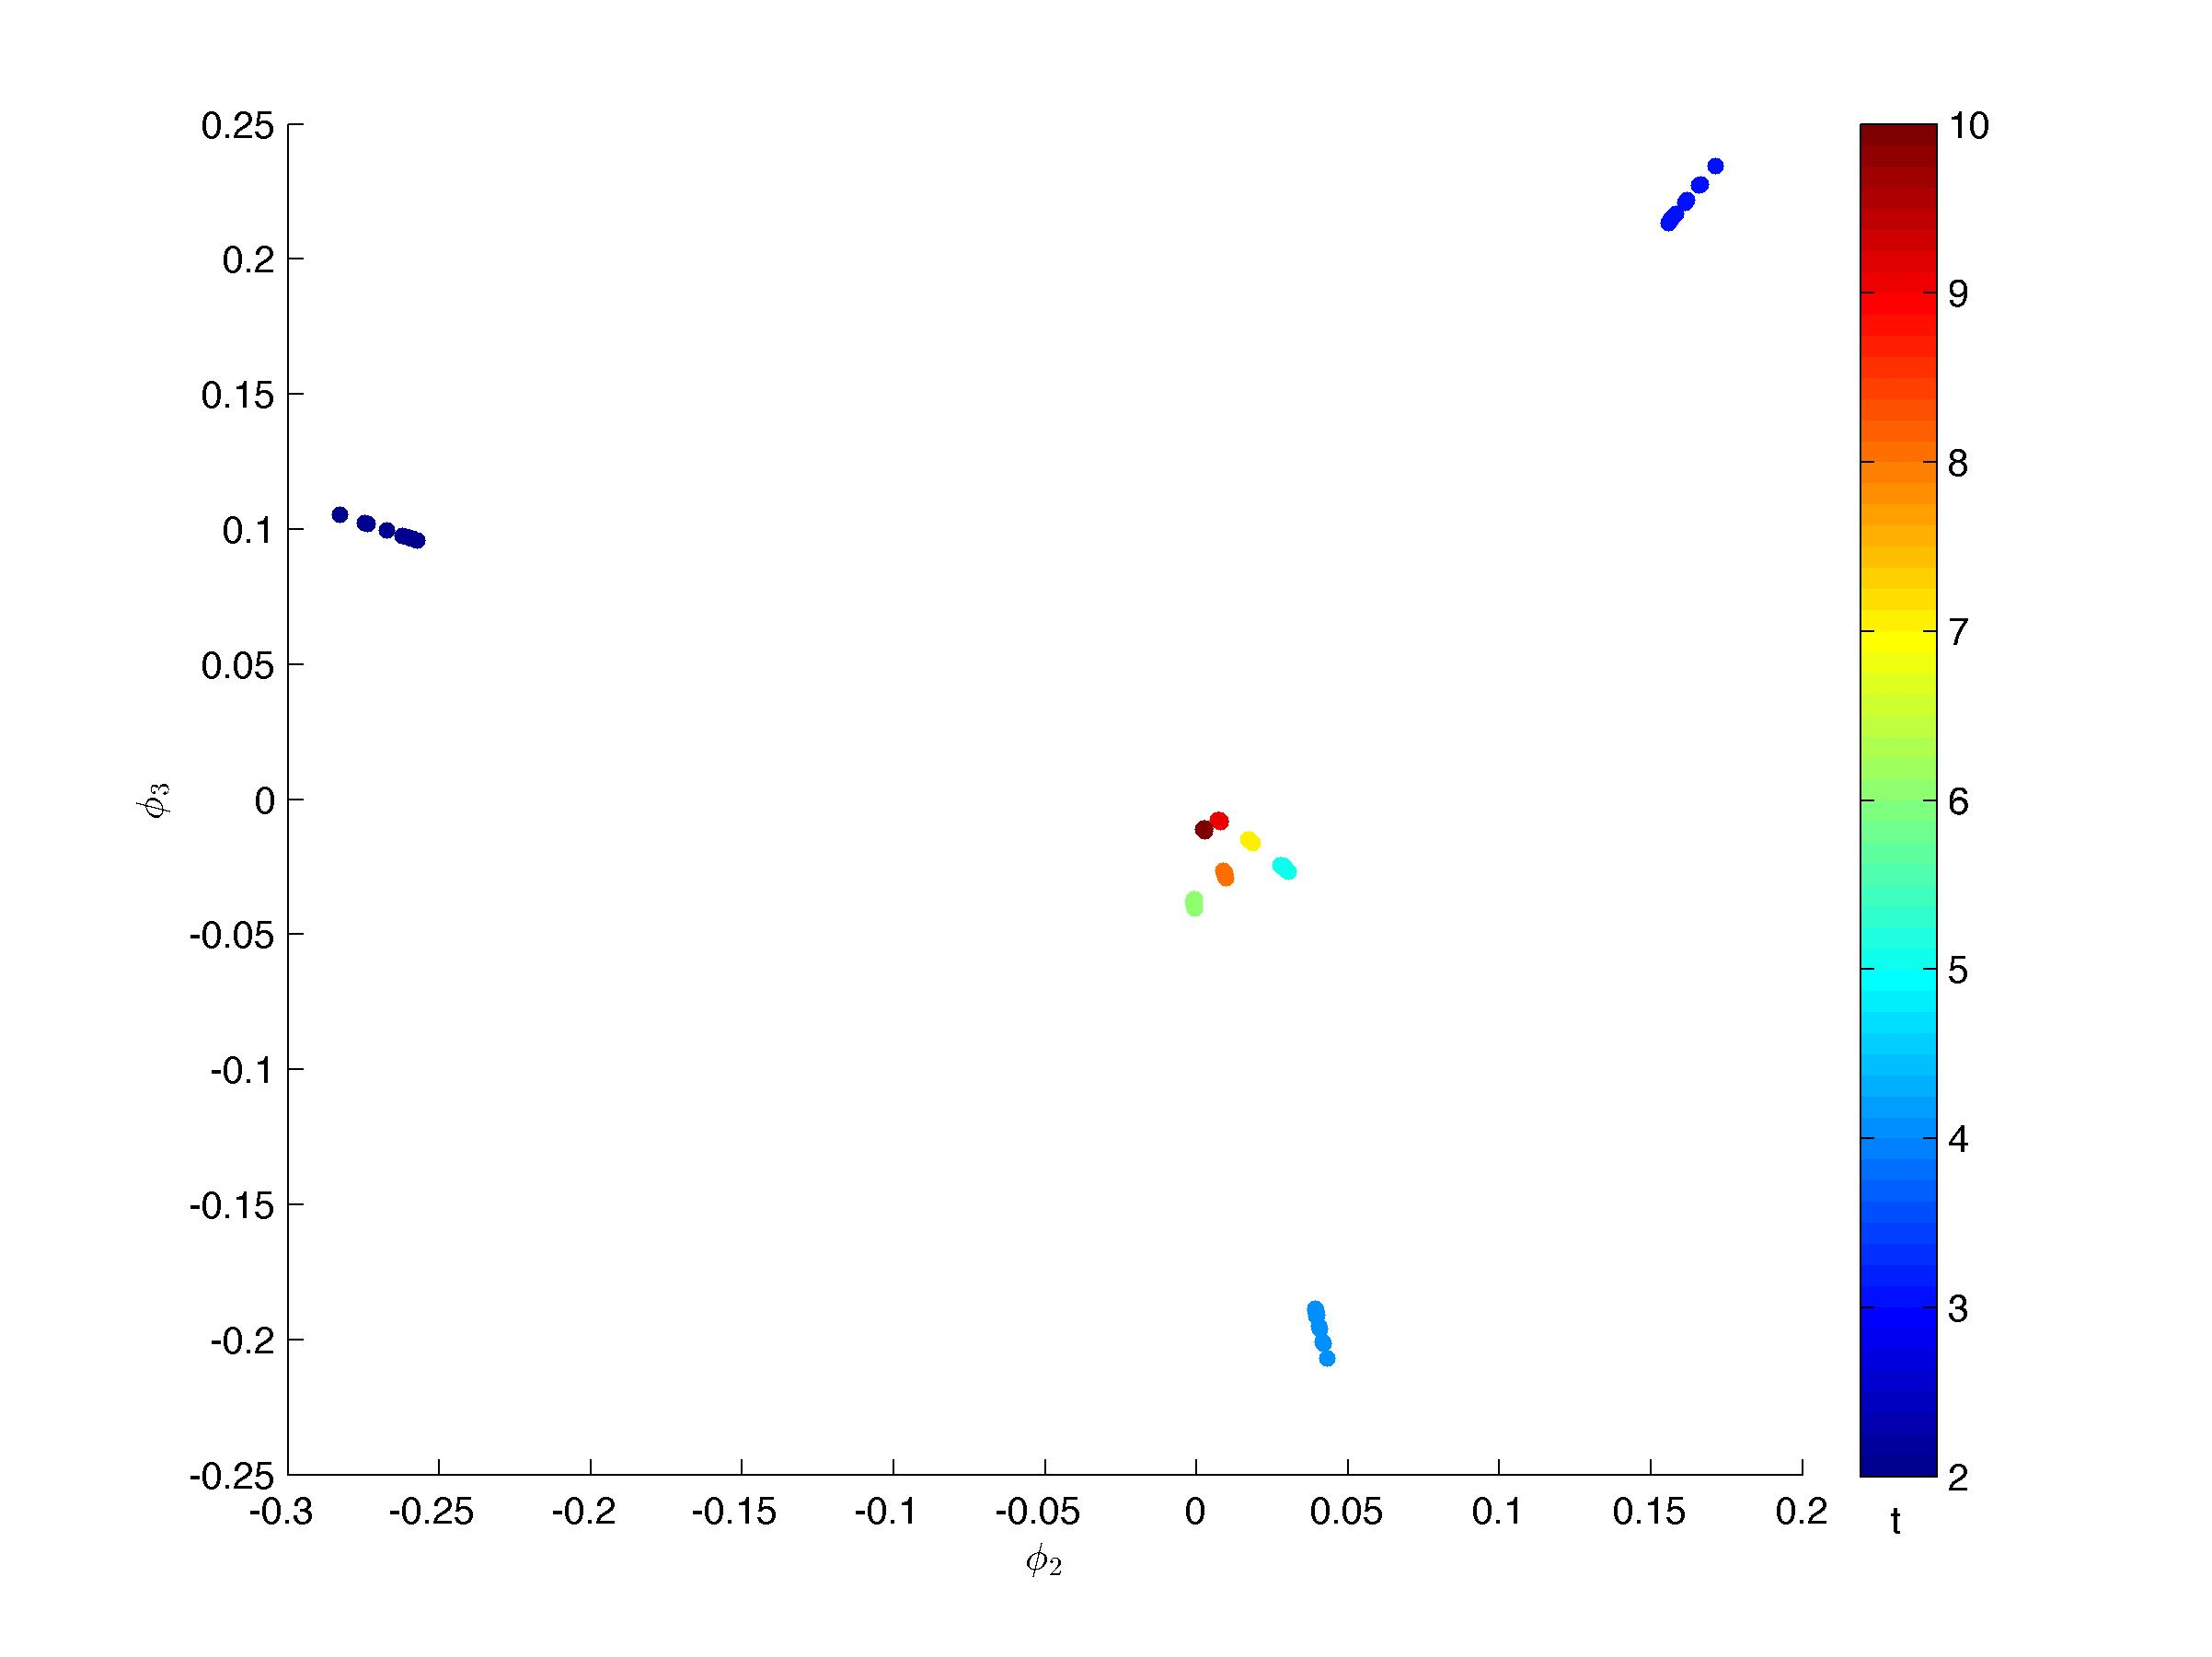
\includegraphics[width=\textwidth]{rawhist_t_1}
\caption{}
\end{subfigure}
\begin{subfigure}{0.5\textwidth}
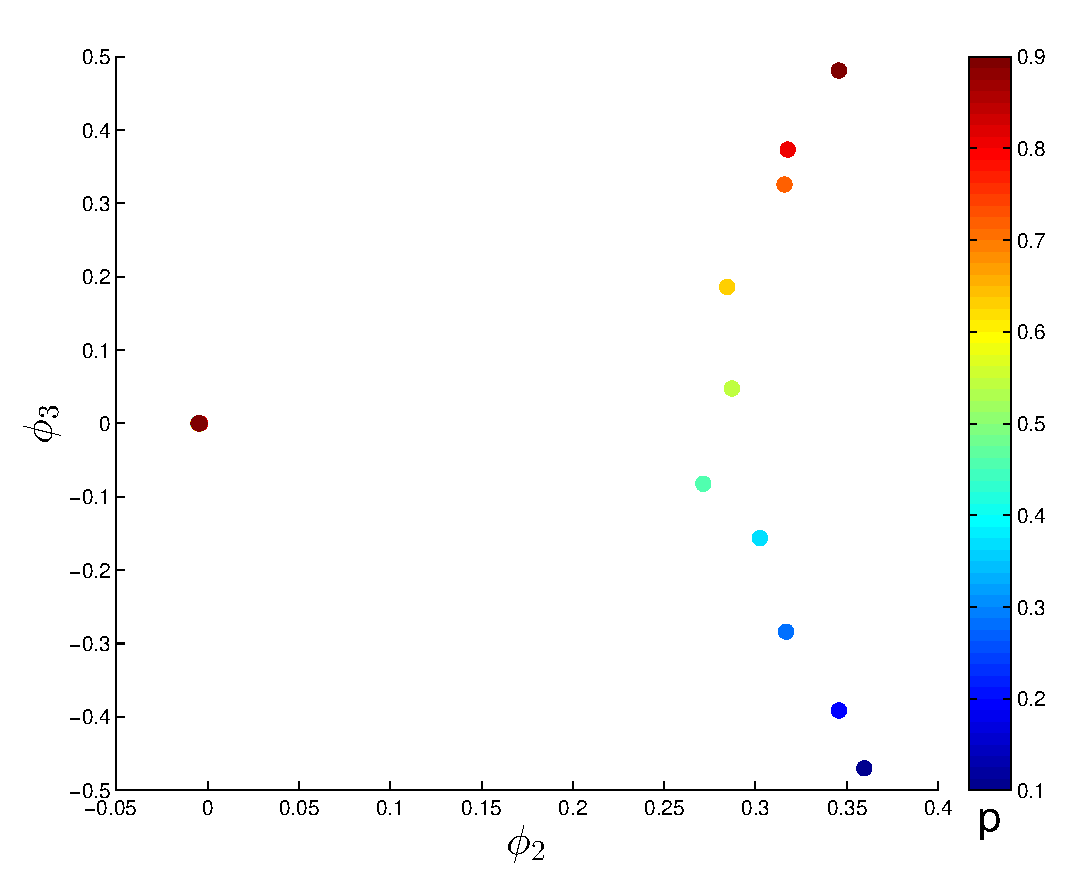
\includegraphics[width=\textwidth]{rawhist_p_400}
\caption{}
\end{subfigure}
\begin{subfigure}{0.5\textwidth}
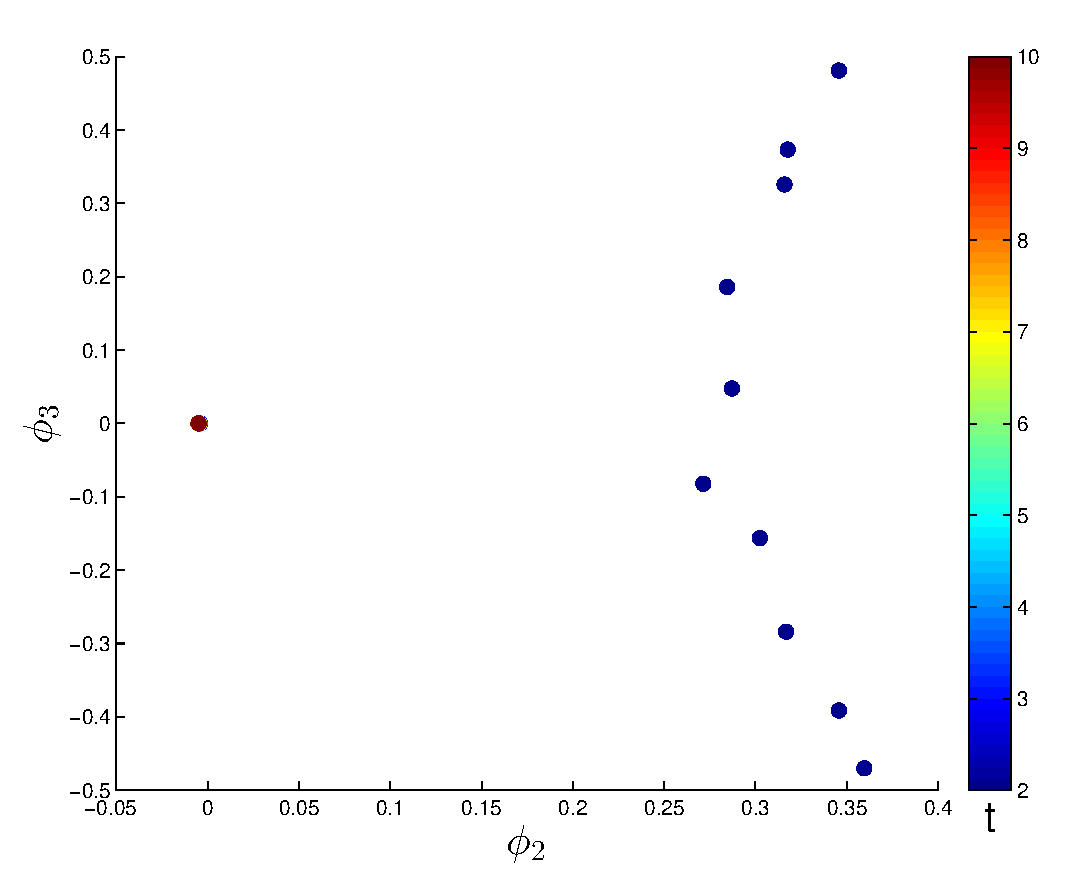
\includegraphics[width=\textwidth]{rawhist_t_400}
\caption{}
\end{subfigure}
\caption{Diffusion maps embeddings computed from simulation data of the velocity jump process with (a,b) $\lambda=1$, $s=1$, and (c,d) $\lambda=400$, $s=20$. The distances used in the diffusion maps kernel are the Euclidean distances between the histograms of particle positions. The data are colored by (a, c) $p$, the initial probability of left--moving particles, and (b, d) $t$, time. The first two diffusion maps modes do not capture any of the important parameters in our simulations.}
\label{fig:dmaps_embed}
\end{figure}

\begin{figure}[htb]
\begin{subfigure}{0.5\textwidth}
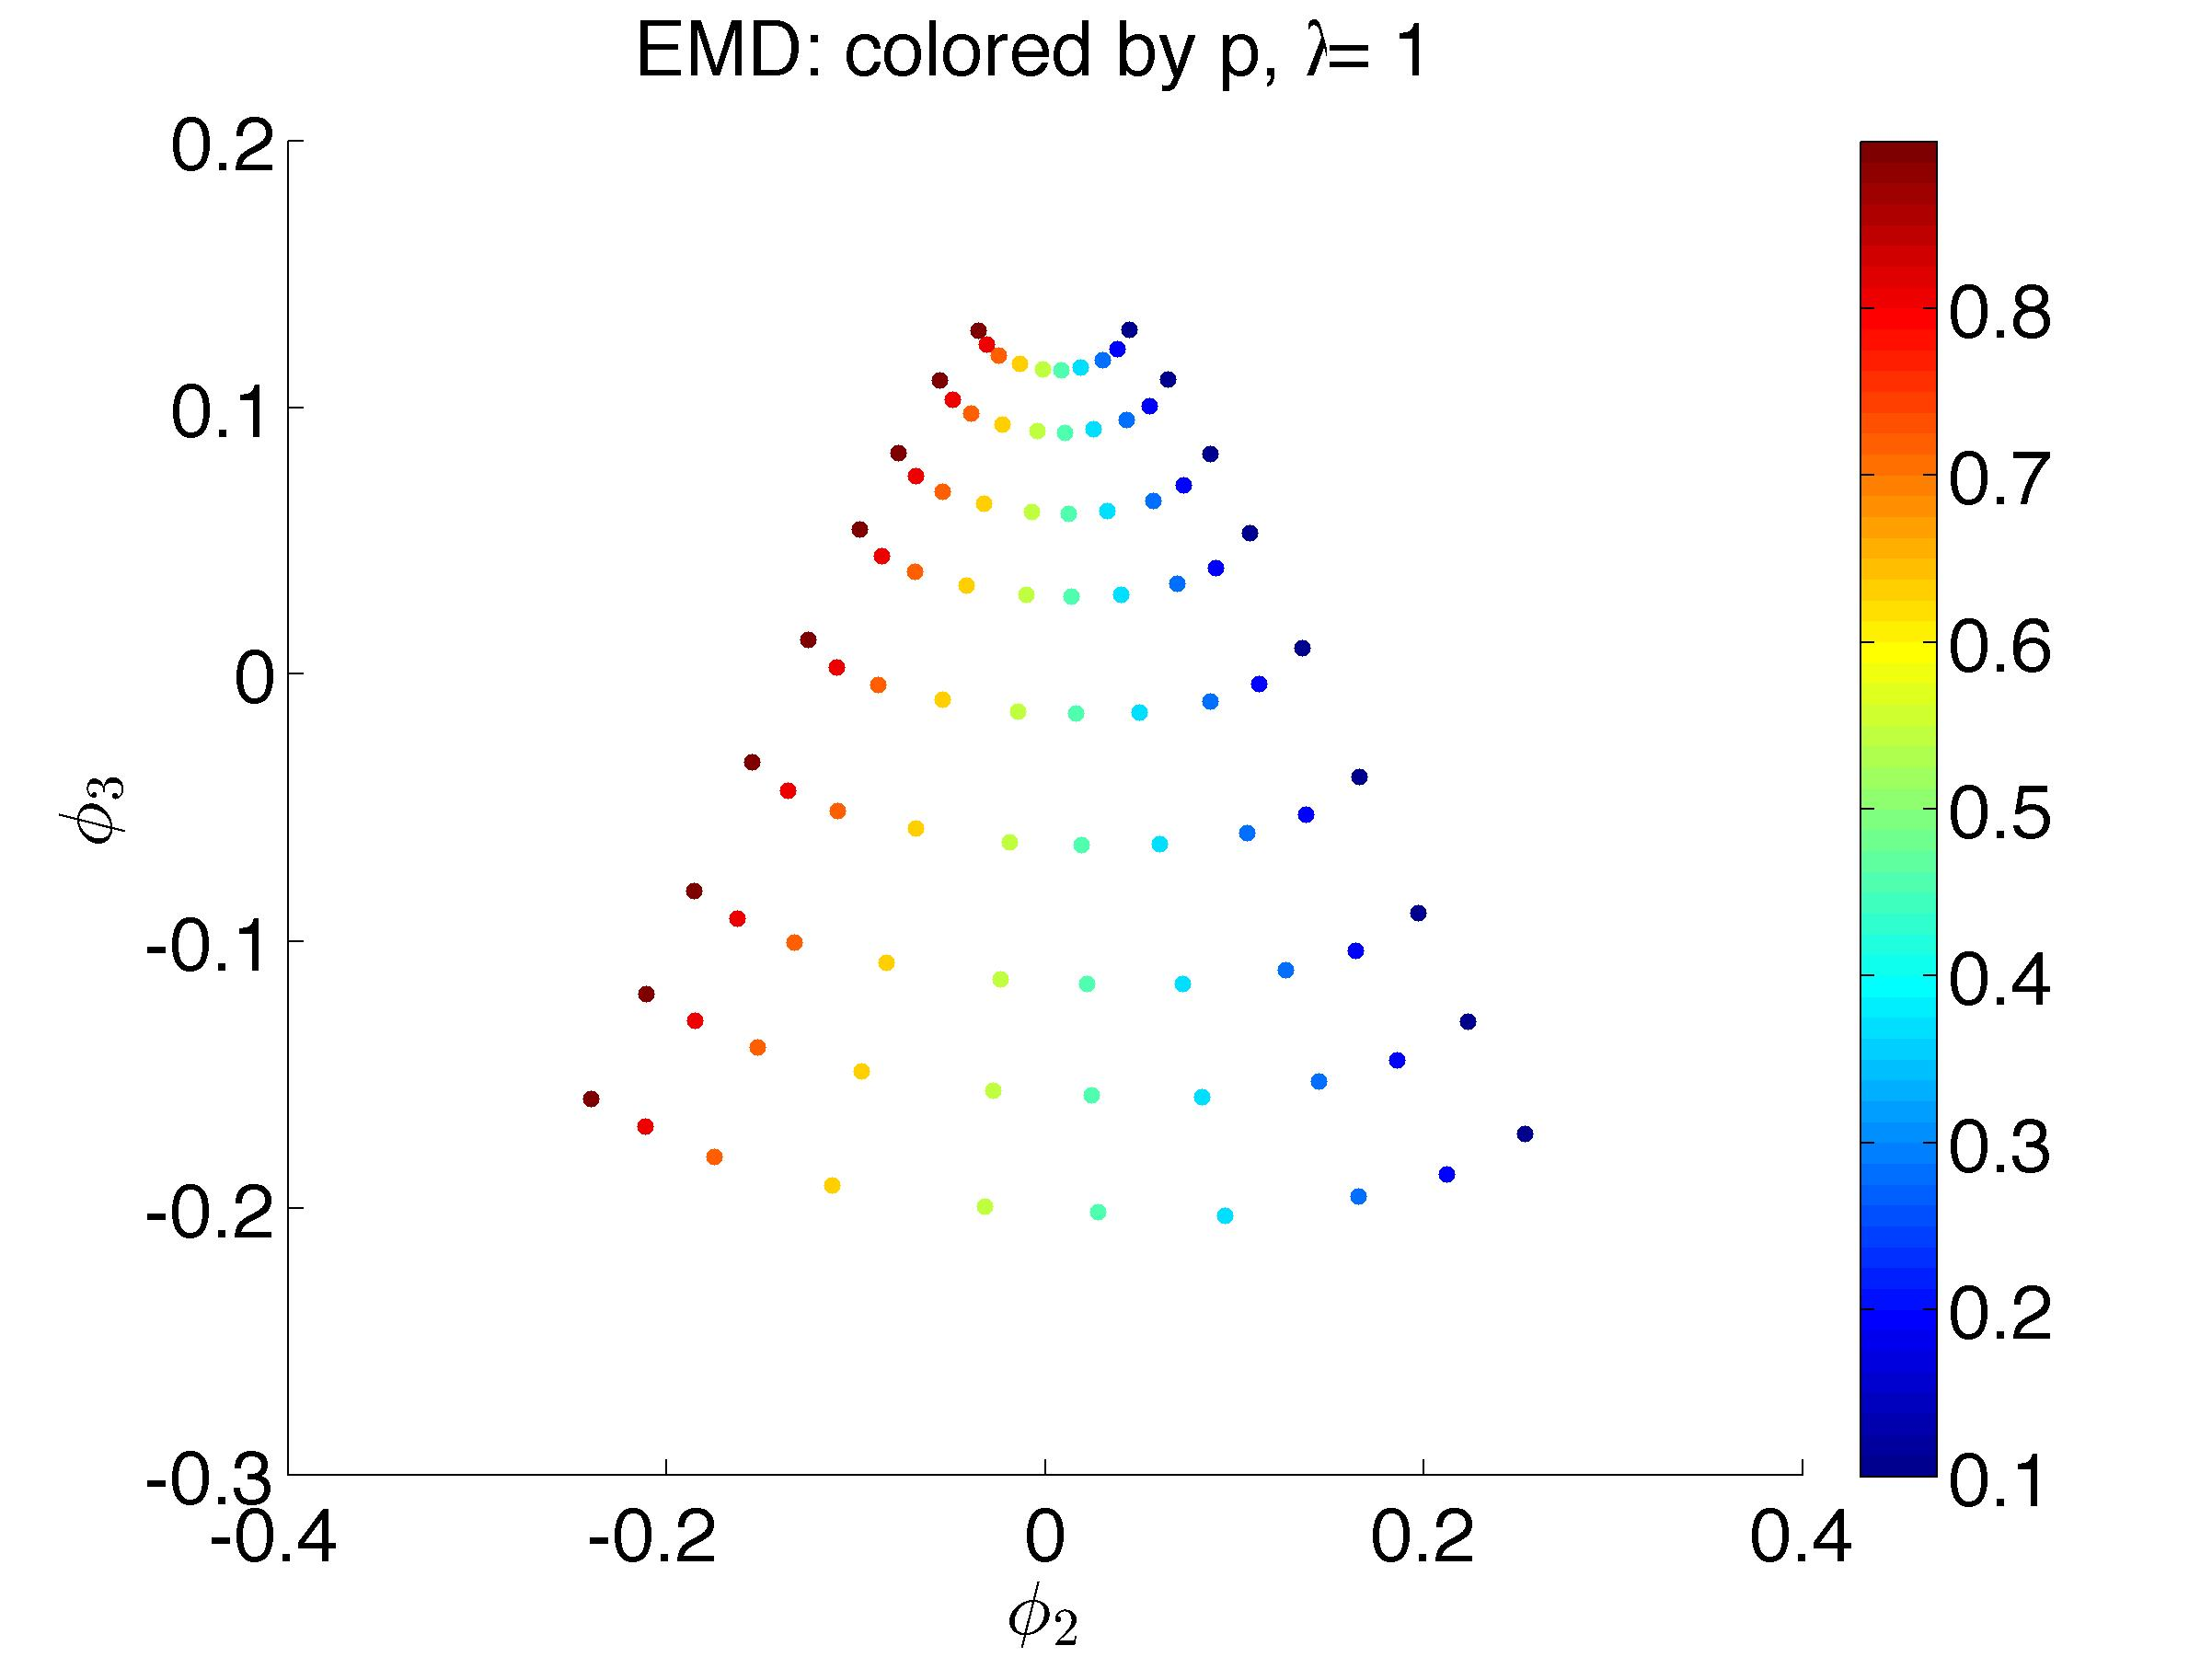
\includegraphics[width=\textwidth]{EMD_p_1}
\caption{}
\end{subfigure}
\begin{subfigure}{0.5\textwidth}
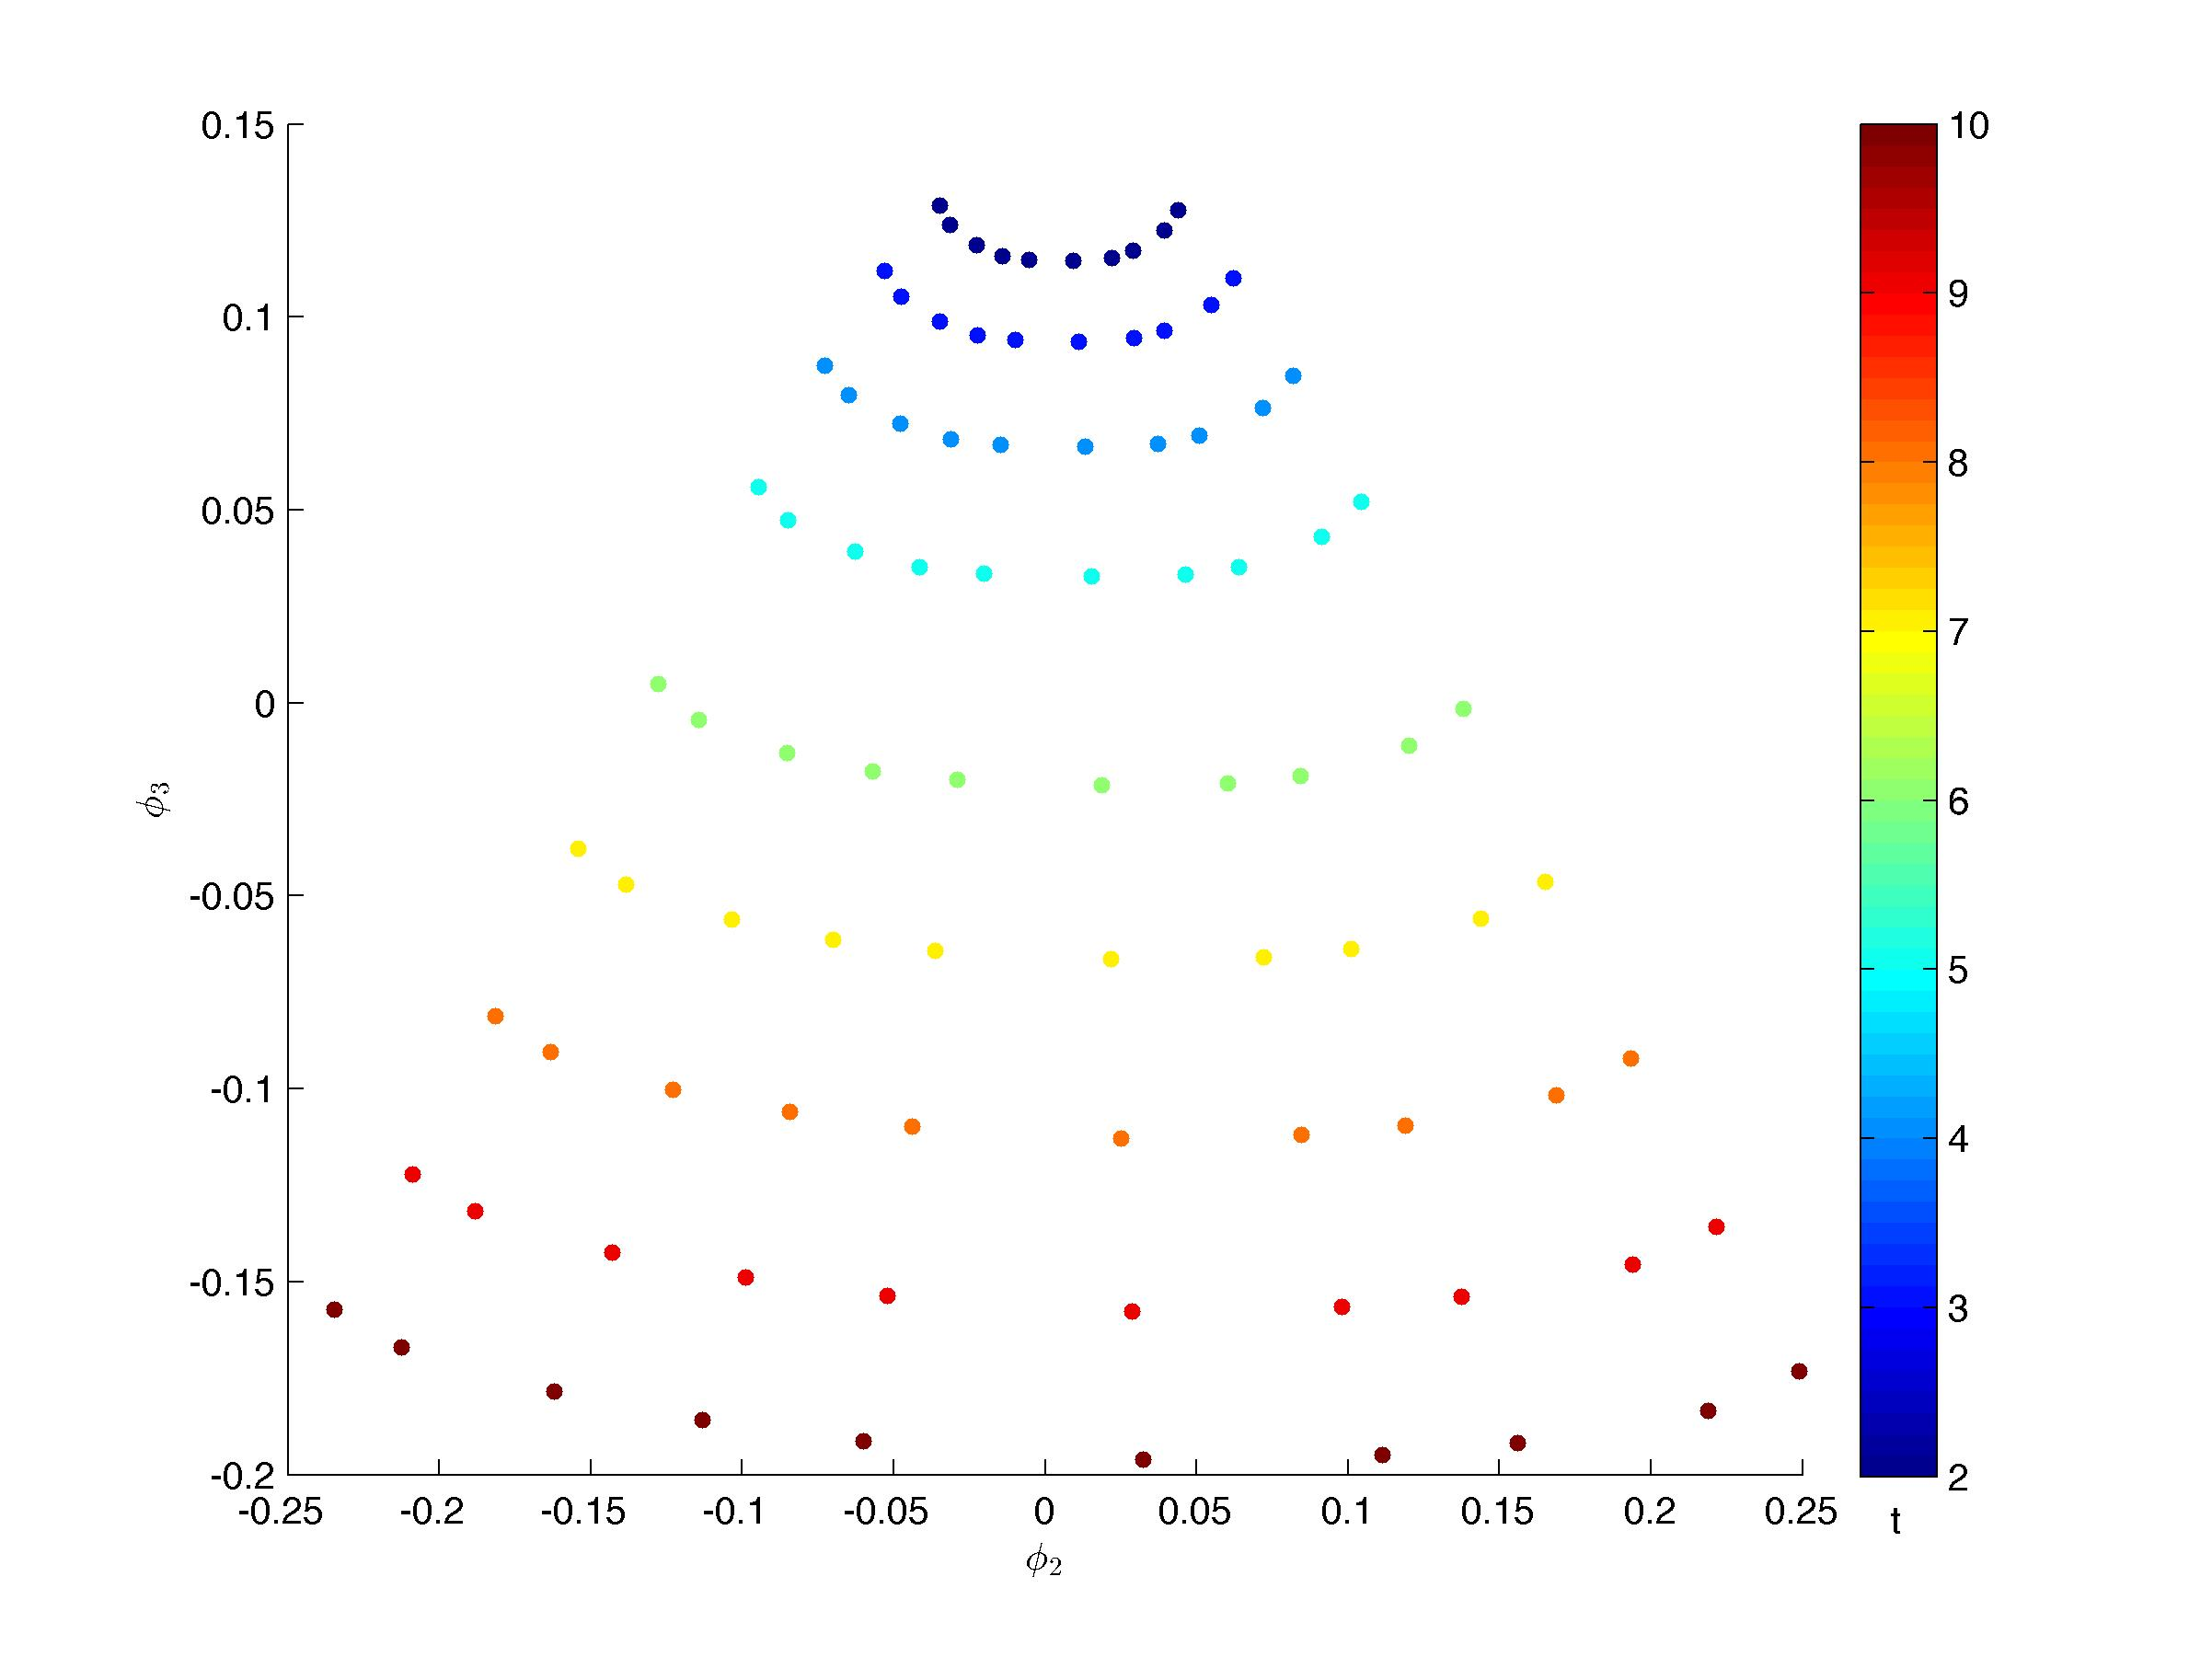
\includegraphics[width=\textwidth]{EMD_t_1}
\caption{}
\end{subfigure}
\begin{subfigure}{0.5\textwidth}
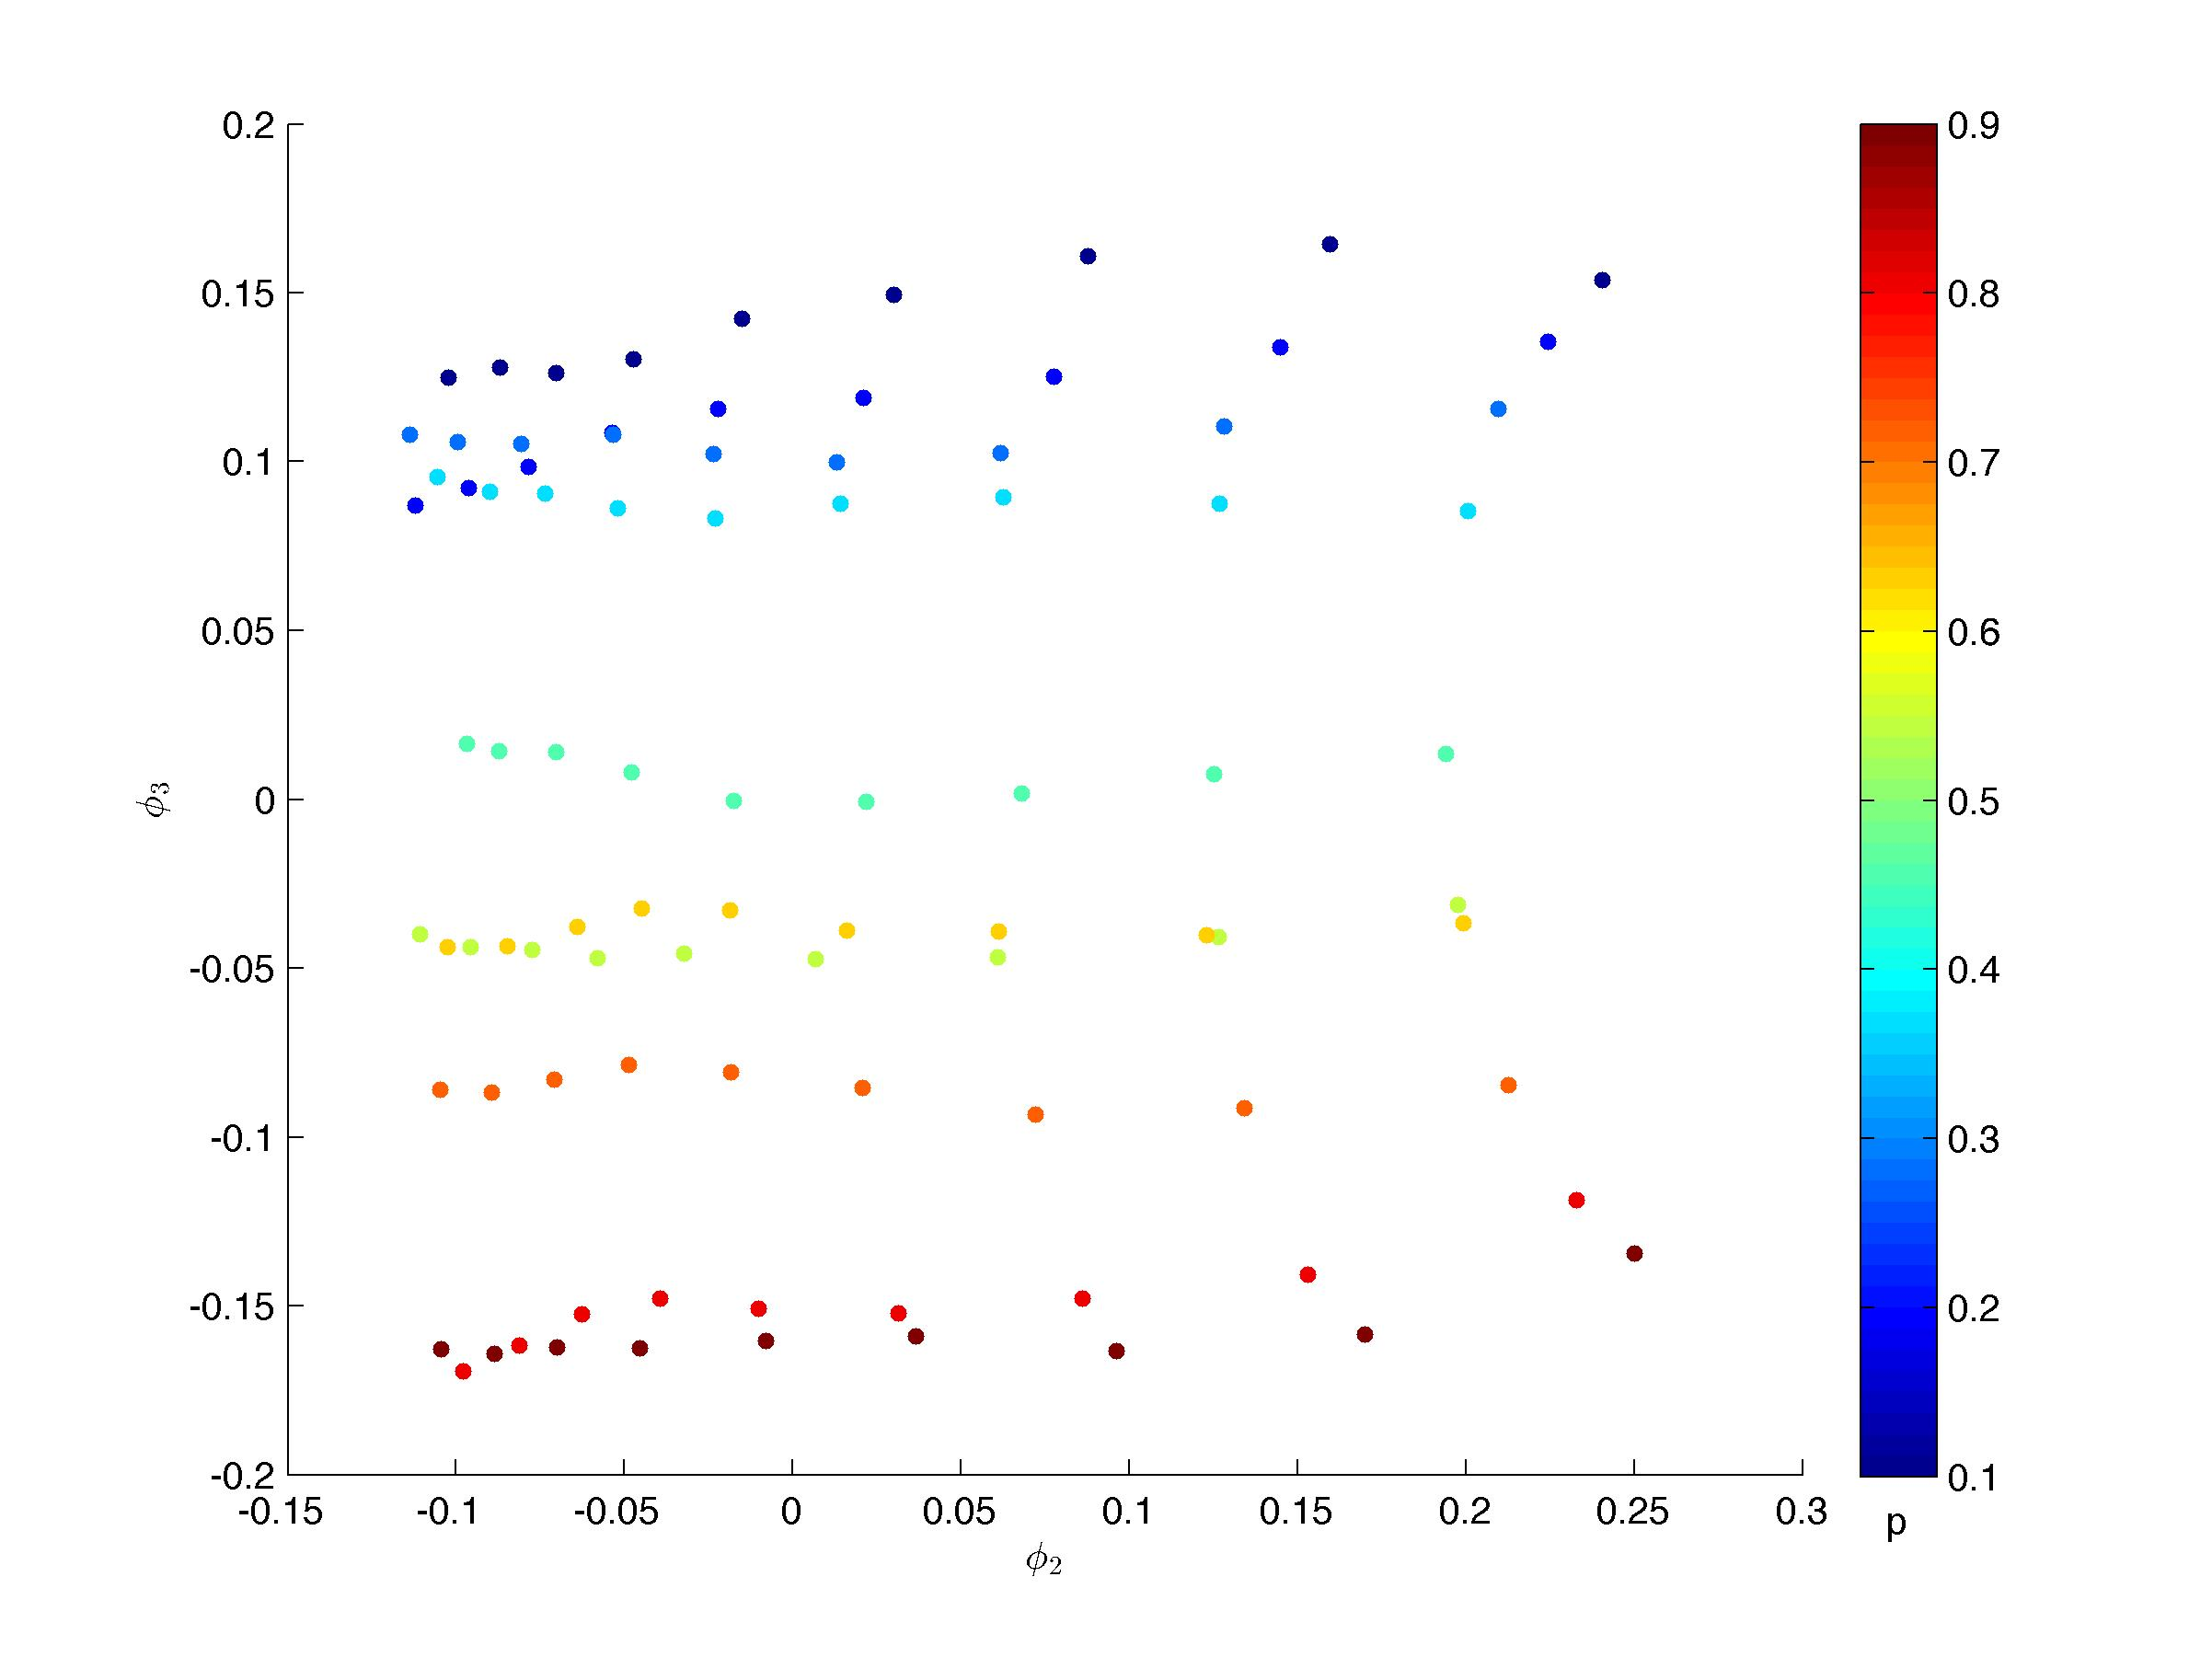
\includegraphics[width=\textwidth]{EMD_p_400}
\caption{}
\end{subfigure}
\begin{subfigure}{0.5\textwidth}
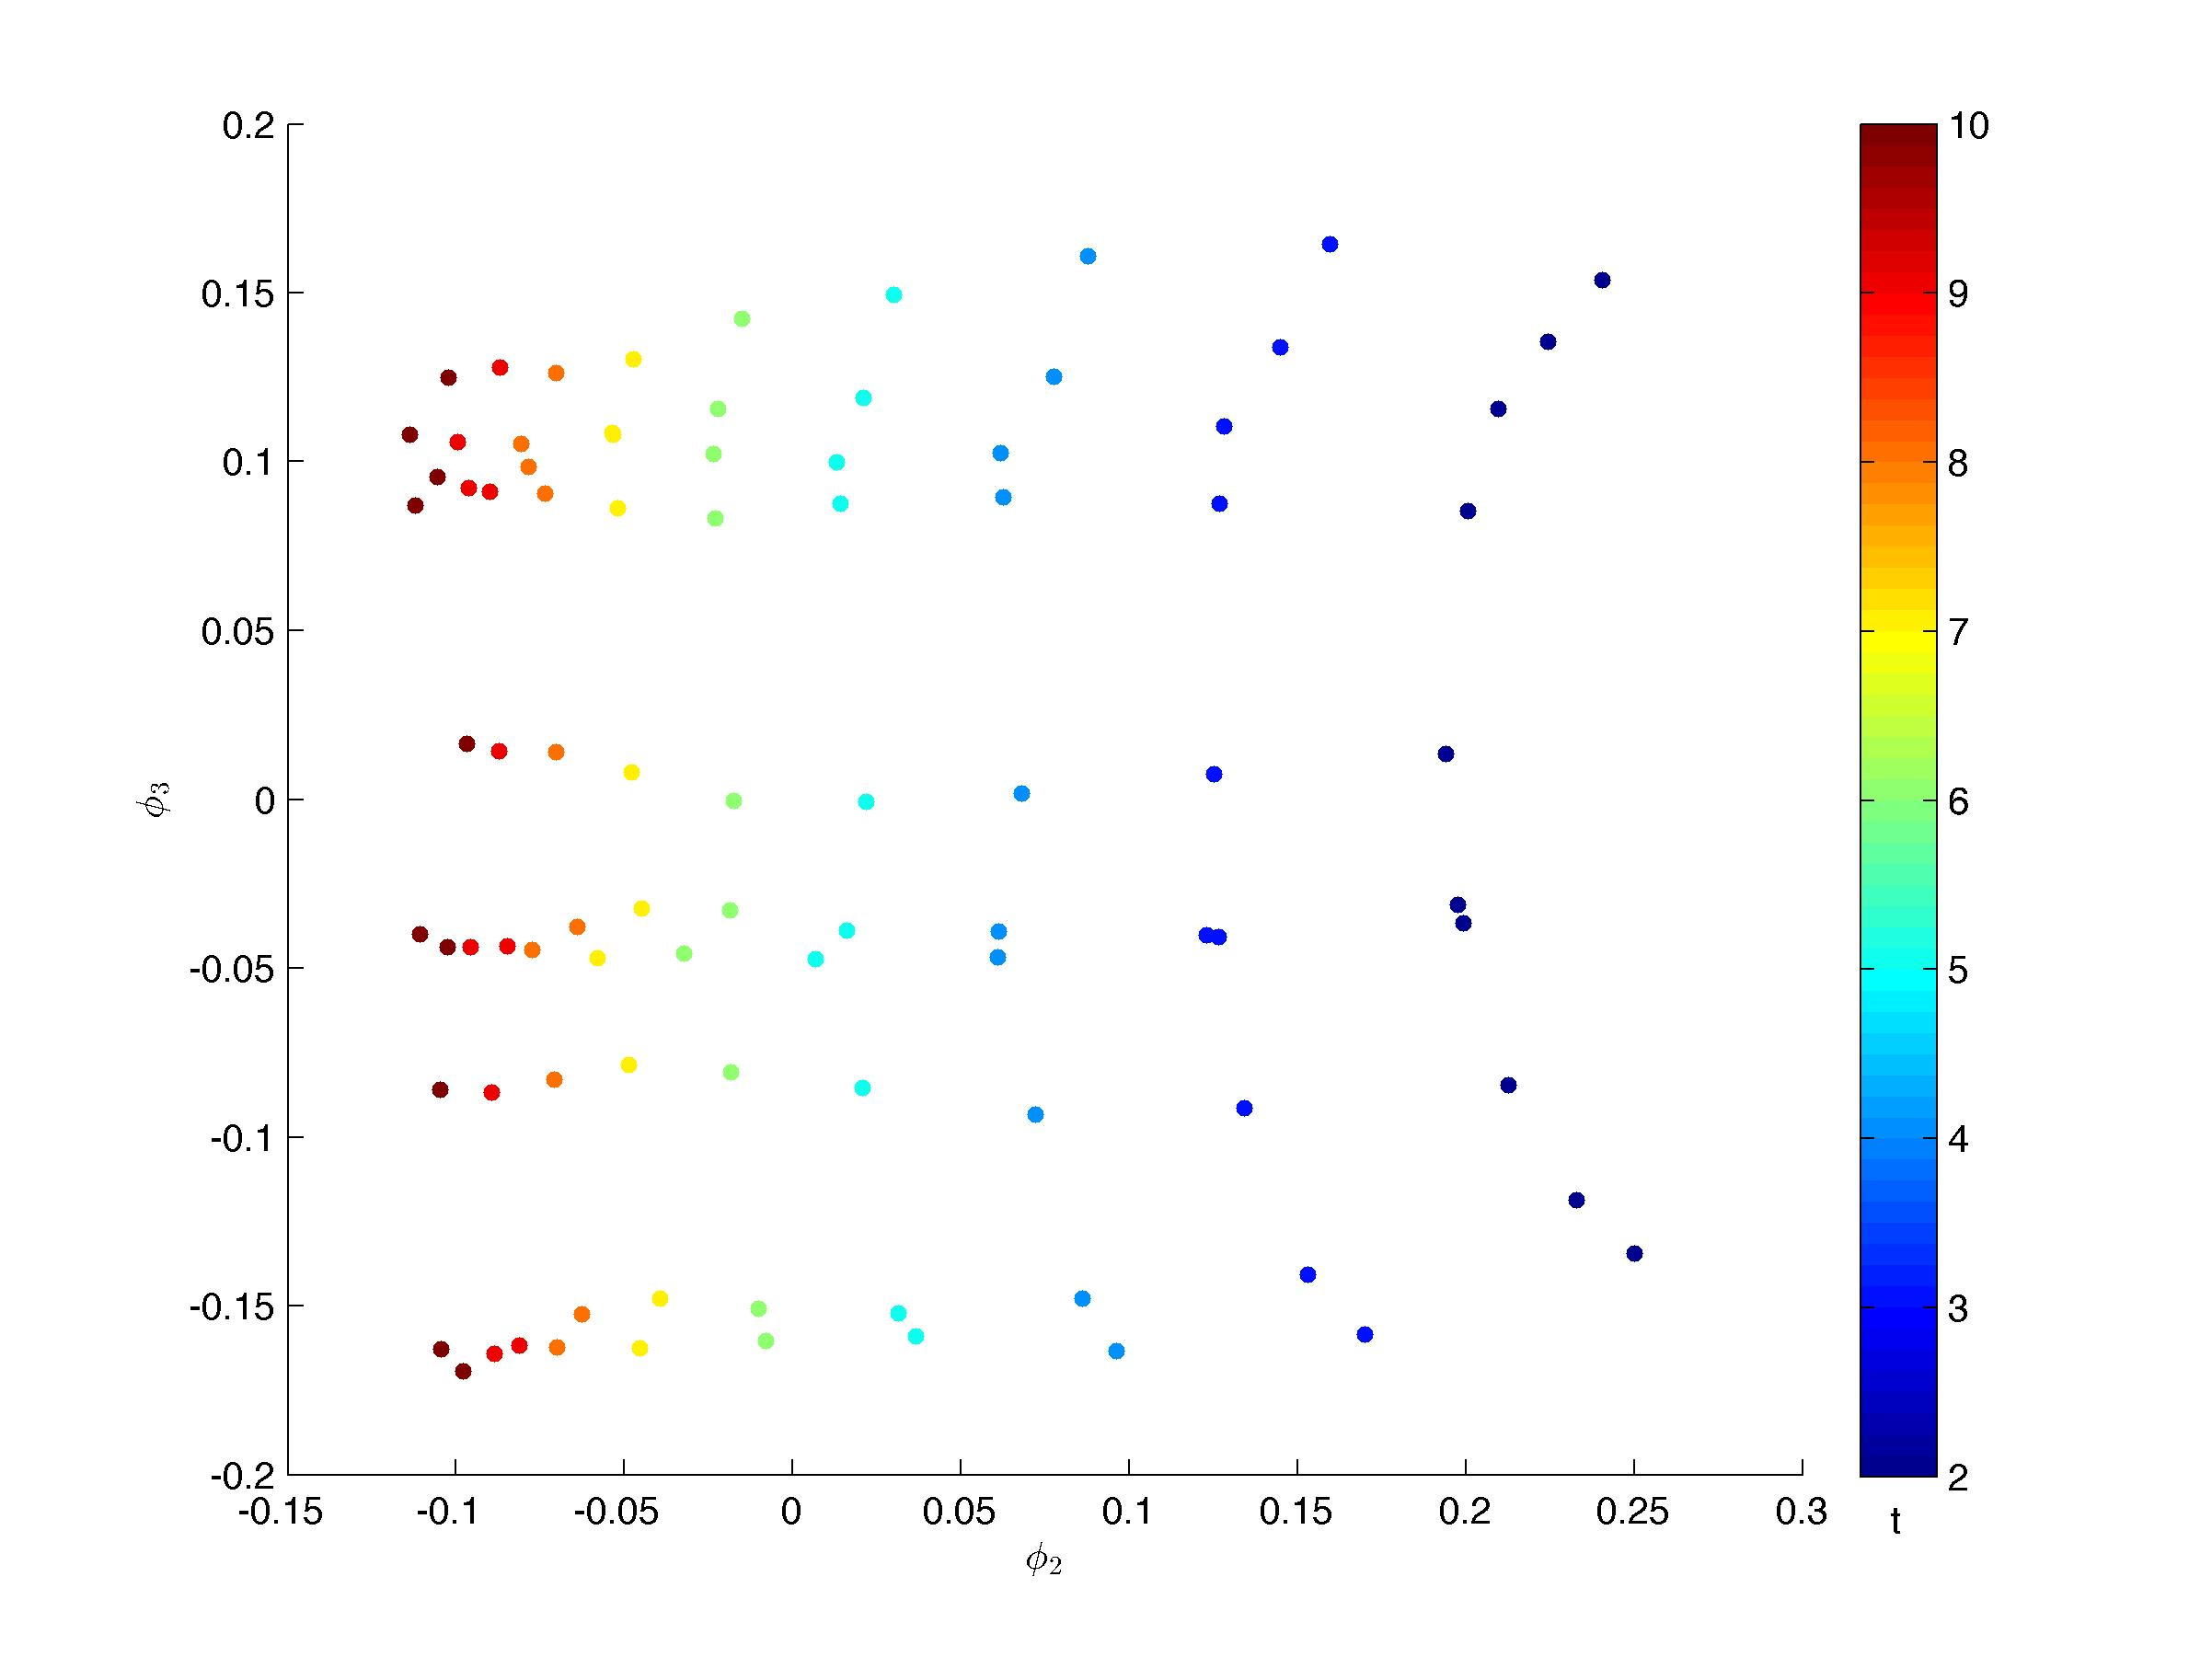
\includegraphics[width=\textwidth]{EMD_t_400}
\caption{}
\end{subfigure}
\caption{Diffusion maps embeddings computed from simulation data of the velocity jump process with (a,b) $\lambda=1$, $s=1$, and (c,d) $\lambda=400$, $s=20$. The distances used in the diffusion maps kernel are the earth mover's distances between the histograms of particle positions. The data are colored by (a, c) $p$, the initial probability of left--moving particles, and (b, d) $t$, time. One can see that these two parameters, $p$ and $t$, are well--correlated with the first two diffusion maps modes, $\phi_2$ and $\phi_3$. However, the ``more important'' mode, $\phi_2$, is correlated with $p$ for the small $\lambda$ case, and correalted with $t$ for the large $\lambda$ case. This is consistent with the asymtotic analysis discussed in Section \ref{subsec:mode_analysis}}
\label{fig:dmaps_embed}
\end{figure}

\end{document}